% Slide: Tổng quan phần mềm Module camera
\begin{frame}{Module camera: Tổng quan phần mềm}
    \begin{block}{Tổng quan}
        \begin{itemize}
            \item Triển khai trên vi điều khiển \textbf{ESP32-S3}.
            \item Thu thập và truyền tải video từ camera \textbf{OV5640} theo thời gian thực.
            \item Cung cấp luồng video MJPEG qua HTTP cho các module xử lý thị giác máy tính.
            \item Dựa trên kiến trúc hướng sự kiện của \textbf{ESP-IDF}, quản lý đồng thời mạng, camera, và bộ đệm.
        \end{itemize}
    \end{block}
    \label{sec:module_ii_software}
\end{frame}

% Slide: Luồng hoạt động chính
\begin{frame}[fragile]{Module camera: Luồng hoạt động chính}
    \begin{block}{Quy trình}
        \begin{enumerate}
            \item \textbf{Khởi tạo hệ thống}: Cấu hình Wi-Fi, camera, và máy chủ HTTP.
            \item \textbf{Chờ yêu cầu client}: Lắng nghe yêu cầu xem video.
            \item \textbf{Lấy khung hình}: Sử dụng triple buffering trên PSRAM để giảm độ trễ.
            \item \textbf{Gửi frame qua HTTP}: Frame JPEG đóng gói trong phản hồi HTTP multipart.
            \item \textbf{Giám sát và xử lý lỗi}: Kiểm tra FPS, xử lý ngắt kết nối client.
        \end{enumerate}
    \end{block}
\end{frame}

% Slide: Sơ đồ luồng hoạt động
\begin{frame}[fragile]{Module camera: Sơ đồ luồng hoạt động}
    \begin{figure}
        \centering
        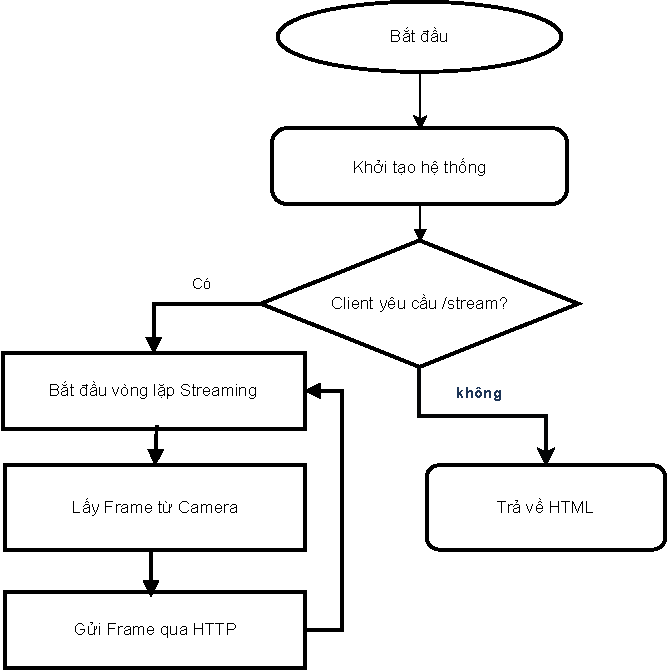
\includegraphics[width=0.85\textwidth,height=0.7\textheight,keepaspectratio]{images/module2_flow_2.pdf}
        \caption{Luồng hoạt động chính của phần mềm Module camera.}
        \label{fig:sw_architecture_flow}
    \end{figure}
\end{frame}

% Slide: Cấu hình phần mềm với Kconfig
\begin{frame}{Module camera: Cấu hình phần mềm với Kconfig}
    \begin{block}{Thông số chính}
        \begin{itemize}
            \item \textbf{Wi-Fi}: SSID và Password để kết nối mạng.
            \item \textbf{Kích thước khung hình}: Từ QQVGA đến UXGA (chất lượng video, băng thông).
            \item \textbf{Chất lượng JPEG}: Giá trị 10–63 (độ nén hình ảnh).
            \item \textbf{Khoảng thời gian giữa các frame}: 0–200 ms (tốc độ khung hình, băng thông).
        \end{itemize}
    \end{block}
\end{frame}

% Slide: Tối ưu hóa hiệu suất và ứng dụng
\begin{frame}{Module camera: Tối ưu hóa hiệu suất và ứng dụng}
    \begin{columns}[t]
        \begin{column}{0.48\textwidth}
            \begin{block}{Kỹ thuật tối ưu}
                \begin{itemize}
                    \item \textbf{Quản lý bộ nhớ}: Sử dụng PSRAM cho buffer, giảm tải SRAM.
                    \item \textbf{Triple buffering}: Chụp frame mới đồng thời với truyền frame cũ.
                    \item \textbf{Giám sát hiệu suất}: Đo FPS thời gian thực, xử lý lỗi ngắt kết nối.
                \end{itemize}
            \end{block}
        \end{column}
        \begin{column}{0.48\textwidth}
            \begin{block}{Ứng dụng}
                \begin{itemize}
                    \item Cầu nối giữa phần cứng và các module xử lý
                    \item Đầu ra video HTTP cho thuật toán thị giác máy tính.
                \end{itemize}
            \end{block}
        \end{column}
    \end{columns}
\end{frame}
